\documentclass{extbook}[14pt]
\usepackage{multicol, enumerate, enumitem, hyperref, color, soul, setspace, parskip, fancyhdr, amssymb, amsthm, amsmath, latexsym, units, mathtools}
\everymath{\displaystyle}
\usepackage[headsep=0.5cm,headheight=0cm, left=1 in,right= 1 in,top= 1 in,bottom= 1 in]{geometry}
\usepackage{dashrule}  % Package to use the command below to create lines between items
\newcommand{\litem}[1]{\item #1

\rule{\textwidth}{0.4pt}}
\pagestyle{fancy}
\lhead{}
\chead{Answer Key for Progress Quiz 3 Version A}
\rhead{}
\lfoot{3012-8528}
\cfoot{}
\rfoot{Summer C 2021}
\begin{document}
\textbf{This key should allow you to understand why you choose the option you did (beyond just getting a question right or wrong). \href{https://xronos.clas.ufl.edu/mac1105spring2020/courseDescriptionAndMisc/Exams/LearningFromResults}{More instructions on how to use this key can be found here}.}

\textbf{If you have a suggestion to make the keys better, \href{https://forms.gle/CZkbZmPbC9XALEE88}{please fill out the short survey here}.}

\textit{Note: This key is auto-generated and may contain issues and/or errors. The keys are reviewed after each exam to ensure grading is done accurately. If there are issues (like duplicate options), they are noted in the offline gradebook. The keys are a work-in-progress to give students as many resources to improve as possible.}

\rule{\textwidth}{0.4pt}

\begin{enumerate}\litem{
Describe the end behavior of the polynomial below.
\[ f(x) = -3(x + 5)^{4}(x - 5)^{7}(x - 7)^{4}(x + 7)^{6} \]The solution is the graph below, which is option A.
    \begin{center}
        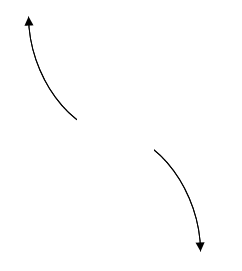
\includegraphics[width=0.3\textwidth]{../Figures/polyEndBehaviorCopyAA.png}
    \end{center}\begin{enumerate}[label=\Alph*.]
\begin{multicols}{2}
\item 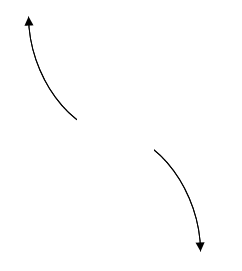
\includegraphics[width = 0.3\textwidth]{../Figures/polyEndBehaviorCopyAA.png}
\item 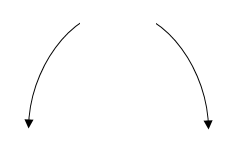
\includegraphics[width = 0.3\textwidth]{../Figures/polyEndBehaviorCopyBA.png}
\item 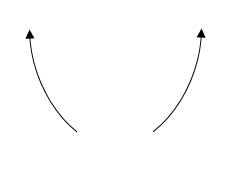
\includegraphics[width = 0.3\textwidth]{../Figures/polyEndBehaviorCopyCA.png}
\item 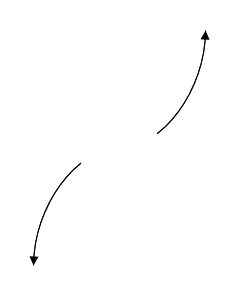
\includegraphics[width = 0.3\textwidth]{../Figures/polyEndBehaviorCopyDA.png}
\end{multicols}\item None of the above.\end{enumerate}
\textbf{General Comment:} Remember that end behavior is determined by the leading coefficient AND whether the \textbf{sum} of the multiplicities is positive or negative.
}
\litem{
Describe the zero behavior of the zero $x = 3$ of the polynomial below.
\[ f(x) = 6(x - 3)^{8}(x + 3)^{13}(x - 4)^{9}(x + 4)^{12} \]The solution is the graph below, which is option B.
    \begin{center}
        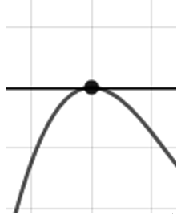
\includegraphics[width=0.3\textwidth]{../Figures/polyZeroBehaviorBA.png}
    \end{center}\begin{enumerate}[label=\Alph*.]
\begin{multicols}{2}
\item 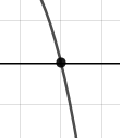
\includegraphics[width = 0.3\textwidth]{../Figures/polyZeroBehaviorAA.png}
\item 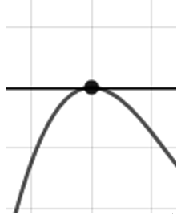
\includegraphics[width = 0.3\textwidth]{../Figures/polyZeroBehaviorBA.png}
\item 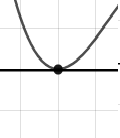
\includegraphics[width = 0.3\textwidth]{../Figures/polyZeroBehaviorCA.png}
\item 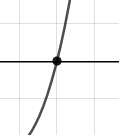
\includegraphics[width = 0.3\textwidth]{../Figures/polyZeroBehaviorDA.png}
\end{multicols}\item None of the above.\end{enumerate}
\textbf{General Comment:} You will need to sketch the entire graph, then zoom in on the zero the question asks about.
}
\litem{
Which of the following equations \textit{could} be of the graph presented below?

\begin{center}
    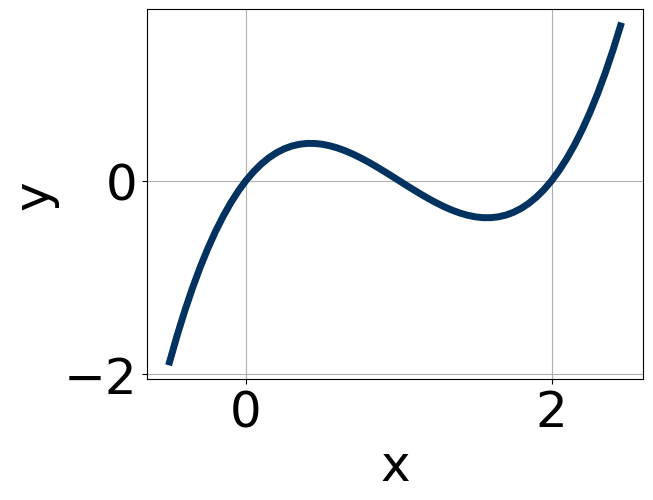
\includegraphics[width=0.5\textwidth]{../Figures/polyGraphToFunctionA.png}
\end{center}


The solution is \( 18x^{7} (x - 2)^{7} (x - 1)^{5} \), which is option C.\begin{enumerate}[label=\Alph*.]
\item \( 4x^{7} (x - 2)^{10} (x - 1)^{5} \)

The factor $2$ should have been an odd power.
\item \( -8x^{9} (x - 2)^{6} (x - 1)^{5} \)

The factor $(x - 2)$ should have an odd power and the leading coefficient should be the opposite sign.
\item \( 18x^{7} (x - 2)^{7} (x - 1)^{5} \)

* This is the correct option.
\item \( 7x^{10} (x - 2)^{8} (x - 1)^{11} \)

The factors $2$ and $0$ have have been odd power.
\item \( -12x^{9} (x - 2)^{5} (x - 1)^{5} \)

This corresponds to the leading coefficient being the opposite value than it should be.
\end{enumerate}

\textbf{General Comment:} General Comments: Draw the x-axis to determine which zeros are touching (and so have even multiplicity) or cross (and have odd multiplicity).
}
\litem{
Construct the lowest-degree polynomial given the zeros below. Then, choose the intervals that contain the coefficients of the polynomial in the form $x^3+bx^2+cx+d$.
\[ 4 + 5 i \text{ and } 2 \]The solution is \( x^{3} -10 x^{2} +57 x -82 \), which is option D.\begin{enumerate}[label=\Alph*.]
\item \( b \in [7, 16], c \in [56, 57.3], \text{ and } d \in [81, 86.3] \)

$x^{3} +10 x^{2} +57 x + 82$, which corresponds to multiplying out $(x-(4 + 5 i))(x-(4 - 5 i))(x + 2)$.
\item \( b \in [0, 2], c \in [-6.8, -1.8], \text{ and } d \in [3.8, 8.5] \)

$x^{3} + x^{2} -6 x + 8$, which corresponds to multiplying out $(x -4)(x -2)$.
\item \( b \in [0, 2], c \in [-8.8, -6.5], \text{ and } d \in [8.4, 13.1] \)

$x^{3} + x^{2} -7 x + 10$, which corresponds to multiplying out $(x -5)(x -2)$.
\item \( b \in [-13, -4], c \in [56, 57.3], \text{ and } d \in [-84.9, -79.5] \)

* $x^{3} -10 x^{2} +57 x -82$, which is the correct option.
\item \( \text{None of the above.} \)

This corresponds to making an unanticipated error or not understanding how to use nonreal complex numbers to create the lowest-degree polynomial. If you chose this and are not sure what you did wrong, please contact the coordinator for help.
\end{enumerate}

\textbf{General Comment:} Remember that the conjugate of $a+bi$ is $a-bi$. Since these zeros always come in pairs, we need to multiply out $(x-(4 + 5 i))(x-(4 - 5 i))(x-(2))$.
}
\litem{
Which of the following equations \textit{could} be of the graph presented below?

\begin{center}
    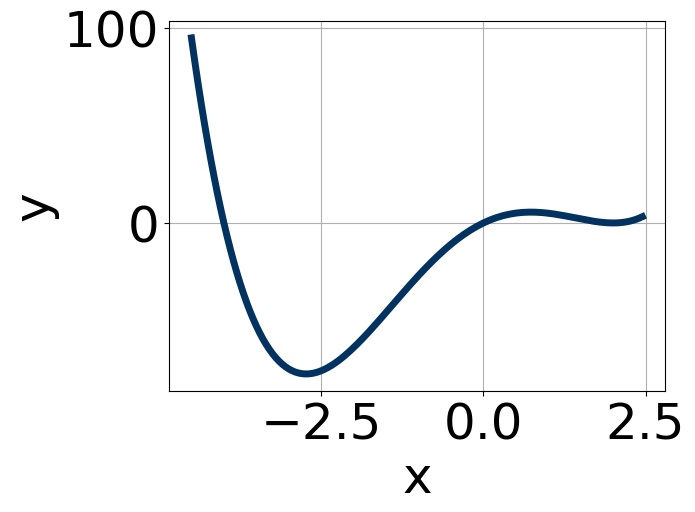
\includegraphics[width=0.5\textwidth]{../Figures/polyGraphToFunctionCopyA.png}
\end{center}


The solution is \( 11x^{9} (x - 2)^{8} (x + 4)^{7} \), which is option D.\begin{enumerate}[label=\Alph*.]
\item \( -18x^{9} (x - 2)^{10} (x + 4)^{8} \)

The factor $(x + 4)$ should have an odd power and the leading coefficient should be the opposite sign.
\item \( 19x^{6} (x - 2)^{9} (x + 4)^{9} \)

The factor $2$ should have an even power and the factor $0$ should have an odd power.
\item \( -14x^{9} (x - 2)^{6} (x + 4)^{5} \)

This corresponds to the leading coefficient being the opposite value than it should be.
\item \( 11x^{9} (x - 2)^{8} (x + 4)^{7} \)

* This is the correct option.
\item \( 19x^{6} (x - 2)^{10} (x + 4)^{9} \)

The factor $x$ should have an odd power.
\end{enumerate}

\textbf{General Comment:} General Comments: Draw the x-axis to determine which zeros are touching (and so have even multiplicity) or cross (and have odd multiplicity).
}
\litem{
Describe the end behavior of the polynomial below.
\[ f(x) = -3(x + 2)^{3}(x - 2)^{8}(x + 6)^{5}(x - 6)^{5} \]The solution is the graph below, which is option A.
    \begin{center}
        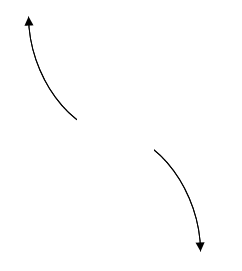
\includegraphics[width=0.3\textwidth]{../Figures/polyEndBehaviorAA.png}
    \end{center}\begin{enumerate}[label=\Alph*.]
\begin{multicols}{2}
\item 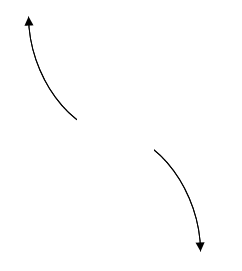
\includegraphics[width = 0.3\textwidth]{../Figures/polyEndBehaviorAA.png}
\item 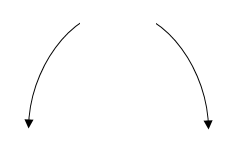
\includegraphics[width = 0.3\textwidth]{../Figures/polyEndBehaviorBA.png}
\item 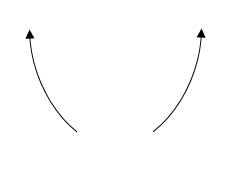
\includegraphics[width = 0.3\textwidth]{../Figures/polyEndBehaviorCA.png}
\item 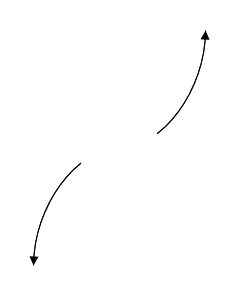
\includegraphics[width = 0.3\textwidth]{../Figures/polyEndBehaviorDA.png}
\end{multicols}\item None of the above.\end{enumerate}
\textbf{General Comment:} Remember that end behavior is determined by the leading coefficient AND whether the \textbf{sum} of the multiplicities is positive or negative.
}
\litem{
Describe the zero behavior of the zero $x = 7$ of the polynomial below.
\[ f(x) = 9(x + 8)^{9}(x - 8)^{7}(x - 7)^{7}(x + 7)^{2} \]The solution is the graph below, which is option A.
    \begin{center}
        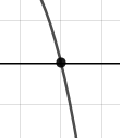
\includegraphics[width=0.3\textwidth]{../Figures/polyZeroBehaviorCopyAA.png}
    \end{center}\begin{enumerate}[label=\Alph*.]
\begin{multicols}{2}
\item 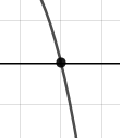
\includegraphics[width = 0.3\textwidth]{../Figures/polyZeroBehaviorCopyAA.png}
\item 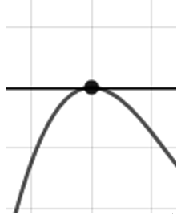
\includegraphics[width = 0.3\textwidth]{../Figures/polyZeroBehaviorCopyBA.png}
\item 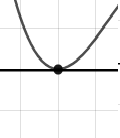
\includegraphics[width = 0.3\textwidth]{../Figures/polyZeroBehaviorCopyCA.png}
\item 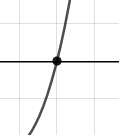
\includegraphics[width = 0.3\textwidth]{../Figures/polyZeroBehaviorCopyDA.png}
\end{multicols}\item None of the above.\end{enumerate}
\textbf{General Comment:} You will need to sketch the entire graph, then zoom in on the zero the question asks about.
}
\litem{
Construct the lowest-degree polynomial given the zeros below. Then, choose the intervals that contain the coefficients of the polynomial in the form $ax^3+bx^2+cx+d$.
\[ \frac{-1}{5}, \frac{-1}{4}, \text{ and } 6 \]The solution is \( 20x^{3} -111 x^{2} -53 x -6 \), which is option E.\begin{enumerate}[label=\Alph*.]
\item \( a \in [16, 21], b \in [107, 116], c \in [-55, -47], \text{ and } d \in [-2, 13] \)

$20x^{3} +111 x^{2} -53 x + 6$, which corresponds to multiplying out $(5x -1)(4x -1)(x + 6)$.
\item \( a \in [16, 21], b \in [-137, -123], c \in [51, 61], \text{ and } d \in [-9, -5] \)

$20x^{3} -129 x^{2} +55 x -6$, which corresponds to multiplying out $(5x -1)(4x -1)(x -6)$.
\item \( a \in [16, 21], b \in [-113, -106], c \in [-55, -47], \text{ and } d \in [-2, 13] \)

$20x^{3} -111 x^{2} -53 x + 6$, which corresponds to multiplying everything correctly except the constant term.
\item \( a \in [16, 21], b \in [-120, -116], c \in [-19, -4], \text{ and } d \in [-2, 13] \)

$20x^{3} -119 x^{2} -7 x + 6$, which corresponds to multiplying out $(5x -1)(4x + 1)(x -6)$.
\item \( a \in [16, 21], b \in [-113, -106], c \in [-55, -47], \text{ and } d \in [-9, -5] \)

* $20x^{3} -111 x^{2} -53 x -6$, which is the correct option.
\end{enumerate}

\textbf{General Comment:} To construct the lowest-degree polynomial, you want to multiply out $(5x + 1)(4x + 1)(x -6)$
}
\litem{
Construct the lowest-degree polynomial given the zeros below. Then, choose the intervals that contain the coefficients of the polynomial in the form $x^3+bx^2+cx+d$.
\[ -5 + 4 i \text{ and } -2 \]The solution is \( x^{3} +12 x^{2} +61 x + 82 \), which is option D.\begin{enumerate}[label=\Alph*.]
\item \( b \in [-14, -10], c \in [53, 67], \text{ and } d \in [-88, -77] \)

$x^{3} -12 x^{2} +61 x -82$, which corresponds to multiplying out $(x-(-5 + 4 i))(x-(-5 - 4 i))(x -2)$.
\item \( b \in [1, 6], c \in [-5, -1], \text{ and } d \in [-8, 0] \)

$x^{3} + x^{2} -2 x -8$, which corresponds to multiplying out $(x -4)(x + 2)$.
\item \( b \in [1, 6], c \in [7, 8], \text{ and } d \in [9, 17] \)

$x^{3} + x^{2} +7 x + 10$, which corresponds to multiplying out $(x + 5)(x + 2)$.
\item \( b \in [9, 25], c \in [53, 67], \text{ and } d \in [82, 90] \)

* $x^{3} +12 x^{2} +61 x + 82$, which is the correct option.
\item \( \text{None of the above.} \)

This corresponds to making an unanticipated error or not understanding how to use nonreal complex numbers to create the lowest-degree polynomial. If you chose this and are not sure what you did wrong, please contact the coordinator for help.
\end{enumerate}

\textbf{General Comment:} Remember that the conjugate of $a+bi$ is $a-bi$. Since these zeros always come in pairs, we need to multiply out $(x-(-5 + 4 i))(x-(-5 - 4 i))(x-(-2))$.
}
\litem{
Construct the lowest-degree polynomial given the zeros below. Then, choose the intervals that contain the coefficients of the polynomial in the form $ax^3+bx^2+cx+d$.
\[ \frac{-5}{4}, \frac{-3}{4}, \text{ and } -5 \]The solution is \( 16x^{3} +112 x^{2} +175 x + 75 \), which is option E.\begin{enumerate}[label=\Alph*.]
\item \( a \in [12, 18], b \in [44, 51], c \in [-145, -143], \text{ and } d \in [73, 83] \)

$16x^{3} +48 x^{2} -145 x + 75$, which corresponds to multiplying out $(4x -5)(4x -3)(x + 5)$.
\item \( a \in [12, 18], b \in [104, 114], c \in [171, 181], \text{ and } d \in [-76, -74] \)

$16x^{3} +112 x^{2} +175 x -75$, which corresponds to multiplying everything correctly except the constant term.
\item \( a \in [12, 18], b \in [72, 73], c \in [-60, -50], \text{ and } d \in [-76, -74] \)

$16x^{3} +72 x^{2} -55 x -75$, which corresponds to multiplying out $(4x -5)(4x + 3)(x + 5)$.
\item \( a \in [12, 18], b \in [-114, -109], c \in [171, 181], \text{ and } d \in [-76, -74] \)

$16x^{3} -112 x^{2} +175 x -75$, which corresponds to multiplying out $(4x -5)(4x -3)(x -5)$.
\item \( a \in [12, 18], b \in [104, 114], c \in [171, 181], \text{ and } d \in [73, 83] \)

* $16x^{3} +112 x^{2} +175 x + 75$, which is the correct option.
\end{enumerate}

\textbf{General Comment:} To construct the lowest-degree polynomial, you want to multiply out $(4x + 5)(4x + 3)(x + 5)$
}
\end{enumerate}

\end{document}